% Template du rapport Locomotion Twin (classe locomotionreport, police Ubuntu).
% Delimiteurs Jinja personnalises (chevrons doubles / chevron-pourcent) pour ne pas
% heurter les accolades LaTeX. Genere par twin_engine.report.render.
% V2 : divulgation progressive (intuition -> detail -> "pour toi"), figures inline,
% textes pedagogiques GENERES depuis les valeurs (cf. report/narrative.py).
\documentclass{locomotionreport}

\renewcommand{\LLCoverLogoPath}{assets/logo_primary_deep}
\renewcommand{\LLHeaderLogoPath}{assets/logo_full_white}

% *Math — macros reprises du thème Beamer Locomotion Lab.
% (amsmath, amssymb, mathtools, bm, stmaryrd sont déjà chargés par la classe.)
\usepackage{nicematrix}
\usepackage{indentfirst}

%\newcommand{\vect}[1]{\text{\bfseries {#1}}}
\newcommand{\vect}[1]{\bm{#1}}
\renewcommand{\d}{\mathrm{d}}
\newcommand{\vmax}{V_{\text{max}}}
\newcommand{\imid}{_{k+\frac{1}{2}}}
\newcommand{\immid}{_{k-\frac{1}{2}}}
\newcommand{\ione}{_{k+1}}
\newcommand{\imone}{_{k-1}}
\newcommand{\none}{^{n+1}}
\newcommand{\odx}[1]{\frac{\partial #1}{\partial x}}
\newcommand{\odxx}[1]{\frac{\partial^2 #1}{\partial x^2}}
\newcommand{\ody}[1]{\frac{\partial #1}{\partial y}}
\newcommand{\odz}[1]{\frac{\partial #1}{\partial z}}
\newcommand{\odt}[1]{\frac{\partial #1}{\partial t}}
\newcommand{\dt}[1]{\frac{\mathrm{d} #1}{\mathrm{d}t}}
\newcommand{\ok}{{\text{K}}}
\newcommand{\inter}{\llbracket 1, N \rrbracket}
\newcommand{\interr}{\llbracket 1, 2N \rrbracket}

\newcommand{\upo}{\bm{\upsilon}^o}
\newcommand{\upe}{\bm{\upsilon}^e}
\newcommand{\upor}{\bm{\upsilon}^o_\Re}
\newcommand{\upoi}{\bm{\upsilon}^o_\Im}
\newcommand{\uper}{\bm{\upsilon}^e_\Re}
\newcommand{\upei}{\bm{\upsilon}^e_\Im}


\newcommand{\A}{\mathcal{A}}
\newcommand{\B}{\mathcal{B}}
\newcommand{\C}{\mathcal{C}}
\newcommand{\Ckk}{\mathcal{C}^{\text{K}}}
\newcommand{\ck}{c^{\text{K}}}
\newcommand{\Ckkk}{\mathcal{C}^{\text{K1}}}

\newcommand{\D}{\mathcal{D}}
\newcommand{\E}{\mathcal{E}}
\newcommand{\F}{\mathcal{F}}
\newcommand{\G}{\mathcal{G}}
\newcommand{\HH}{\mathcal{H}}
\newcommand{\II}{\mathcal{I}}
\newcommand{\J}{\mathcal{J}}
\newcommand{\K}{\mathcal{K}}
\newcommand{\LL}{\mathcal{L}}
\newcommand{\M}{\mathcal{M}}
\newcommand{\N}{\mathcal{N}}
\newcommand{\OO}{\mathcal{O}}
\newcommand{\PP}{\mathcal{P}}
\newcommand{\QQ}{\mathcal{Q}}
\newcommand{\R}{\mathcal{R}}
\newcommand{\SSS}{\mathcal{S}}
\newcommand{\T}{\mathcal{T}}
\newcommand{\U}{\mathcal{U}}
\newcommand{\V}{\mathcal{V}}
\newcommand{\W}{\mathcal{W}}
\newcommand{\X}{\mathcal{X}}
\newcommand{\Y}{\mathcal{Y}}
\newcommand{\Z}{\mathcal{Z}}

\newcommand{\Gv}{\bm{G}}
\newcommand{\Rv}{\bm{R}}
\newcommand{\bv}{\bm{b}}
\newcommand{\q}{\bm{q}}
\newcommand{\qb}{\bm{q}_b}
\newcommand{\qp}{\bm{q}'}
\newcommand{\qh}{\widehat{\bm{q}}}
\newcommand{\qt}{\widetilde{\bm{q}}}
\newcommand{\Q}{\bm{Q}}
\newcommand{\Qb}{\bm{Q}_b}
\newcommand{\Qp}{\bm{Q}'}
\newcommand{\Qh}{\widehat{\bm{Q}}}
\newcommand{\Qt}{\widetilde{\bm{Q}}}
\newcommand{\Wv}{\bm{W}}
\newcommand{\Wb}{\bm{W}_b}
\newcommand{\Wp}{\bm{W}'}
\newcommand{\Wh}{\widehat{\bm{W}}}
%\newcommand{\Wt}{\widetilde{\bm{W}}}
\newcommand{\Wt}{\widehat{\bm{W}}^\dagger}
%\newcommand{\f}{\bm{F}}
%\newcommand{\fh}{\bm{\widehat{F}}}
\newcommand{\f}{\bm{\Phi}}
\newcommand{\fh}{\bm{\widehat{\Phi}}}
\newcommand{\g}{\bm{g}}
\newcommand{\uu}{\bm{u}}
\newcommand{\uh}{\bm{\widehat{u}}}
\newcommand{\rv}{\bm{r}}
\newcommand{\Xv}{\bm{X}}
\newcommand{\xv}{\bm{x}}
\newcommand{\xvr}{\bm{x}_{\Re}}
\newcommand{\xvi}{\bm{x}_{\Im}}
\newcommand{\vv}{\bm{v}}
\newcommand{\vvr}{\bm{v}_{\Re}}
\newcommand{\vvi}{\bm{v}_{\Im}}
\newcommand{\ww}{\bm{w}}
\newcommand{\wh}{\widehat{\bm{w}}}
\newcommand{\wpp}{\bm{w}'}
\newcommand{\vvt}{\bm{\widetilde{v}}}
\newcommand{\wwt}{\bm{\widetilde{w}}}
\newcommand{\yv}{\bm{y}}
\newcommand{\zv}{\bm{z}}
\newcommand{\uodd}{\bm{u}^o}
\newcommand{\ueven}{\bm{u}^e}
\newcommand{\hh}{\hat{\bm{h}}}
\newcommand{\bh}{\hat{\bm{b}}}
\newcommand{\oof}{\text{F}}
\newcommand{\oob}{\text{B}}

\newcommand{\snl}{\sigma^{\text{NL}}}
\newcommand{\stnl}{\text{St}^{\text{NL}}}

\newcommand{\CFL}{\text{CFL}}
\newcommand{\RE}{\text{Re}}
\newcommand{\PR}{\text{Pr}}
\newcommand{\MA}{\text{M}}
\newcommand{\ST}{\text{ST}}

\newcommand{\Sp}{\text{Sp}}

\newcommand*{\tensor}[1]{\overline{\overline{#1}}}

%\floatname{algorithm}{Algorithme}
% Adapté : ne redéfinir que si le paquet algorithmic/algorithmicx est chargé.
\ifdefined\algorithmicrequire
  \renewcommand{\algorithmicrequire}{\textbf{Input:}}
  \renewcommand{\algorithmicensure}{\textbf{Output:}}
\fi

\usepackage{float}      % specificateur [H] : figures placees exactement (inline, pas de flottement)
\captionsetup{justification=centering, singlelinecheck=false}  % legendes centrees
\addbibresource{references.bib}

\newcommand{\Deq}{D_{\mathrm{eq}}}
\newcommand{\VC}{\mathrm{VC}}

\title{Plan de pacing personnalis\'e}
\subtitle{Nice Côte d'Azur by UTMB · 100M \textperiodcentered{} 167\,km \textperiodcentered{} 8\,874\,m\,D+}
\author{The Locomotion Lab}
\date{01/01/2026}
\reporttype{Rapport d'analyse \textperiodcentered{} Locomotion Twin}
\reportref{LL-TWIN}
\reportversion{v1.0}
\reportclient{athlète}

\begin{document}

\makecover

\begin{llabstract}
Ce rapport construit \textbf{ton plan d'allure individualis\'e} pour Nice Côte d'Azur by UTMB · 100M
(167\,km, 8\,874\,m\,D+) \`a partir de deux sources : la trace GPX du parcours et
tes fichiers d'entra\^inement (419~activit\'es de course exploit\'ees). La cha\^ine
\emph{Locomotion Twin} estime ton profil physiologique --- vitesse critique, exposant d'endurance,
durabilit\'e --- puis le confronte au co\^ut \'energ\'etique de la pente pour pr\'edire ton temps
d'arriv\'ee et r\'epartir l'effort. La pr\'ediction centrale est de \textbf{30\,h\,44}
(intervalle 80\,\% : 29\,h\,29 -- 32\,h\,09).
La m\'ethode est valid\'ee \emph{hors \'echantillon} sur tes propres ultras, avec une
erreur moyenne de \textbf{3,4\,\%}.\keywords{pacing \textperiodcentered{} ultra-trail \textperiodcentered{} vitesse critique \textperiodcentered{} durabilit\'e \textperiodcentered{} incertitude}
\end{llabstract}

\LLtoc
\clearpage

% =====================================================================
\section{Synth\`ese}

Ton profil est nettement \textbf{endurant} : ton moteur est calibré pour les très longues durées — c'est le terrain de jeu d'un ultra. Ta r\'esistance \`a la fatigue est \textbf{bonne} (21\,\% de perte d'efficacit\'e en fin de longue sortie) : tu tiens bien la distance, avec une usure progressive maîtrisée. On pr\'edit ton arriv\'ee autour de \textbf{30\,h\,44}, \`a seulement \textbf{64\,\%} de ta vitesse critique : ta vitesse pure n'est jamais la limite, ce sont l'endurance, la durabilit\'e et le ravitaillement qui d\'ecideront. On d\'ecoupe ensuite l'effort segment par segment, avec des fen\^etres horaires.

\begin{llnote}[L'essentiel]
\textbf{Temps d'arriv\'ee pr\'edit : 30\,h\,44}, d\'epart vendredi 25 septembre 2026 à 13h00.
Intervalle de confiance \`a 80\,\% : \textbf{29\,h\,29 -- 32\,h\,09}.
\\[2pt]
\textbf{Intensit\'e cible : $\approx$\,64\,\% de ta vitesse critique}, soutenue
avec une d\'erive ma\^itris\'ee. \`A cette intensit\'e, le facteur limitant n'est pas la
r\'eserve ana\'erobie mais la \textbf{durabilit\'e} et le \textbf{ravitaillement}.\\[2pt]
\textbf{Nuit} : frontale n\'ecessaire du \textbf{km\,38} au \textbf{km\,94} environ.\end{llnote}

Mod\`ele de pr\'ediction employ\'e : \emph{régression personnelle sur tes vrais ultras}. Chaque chiffre d\'ecoule de tes fichiers
ou de la trace officielle, jamais \og~au jug\'e~\fg.

% =====================================================================
\section{Le parcours et ses exigences}

Ta course fait \textbf{167\,km} pour \textbf{8\,874\,m\,D+} et
\textbf{10\,461\,m\,D--}, d\'ecoup\'ee en 16~segments inter-ravitaillements.

\begin{figure}[H]
  \centering
  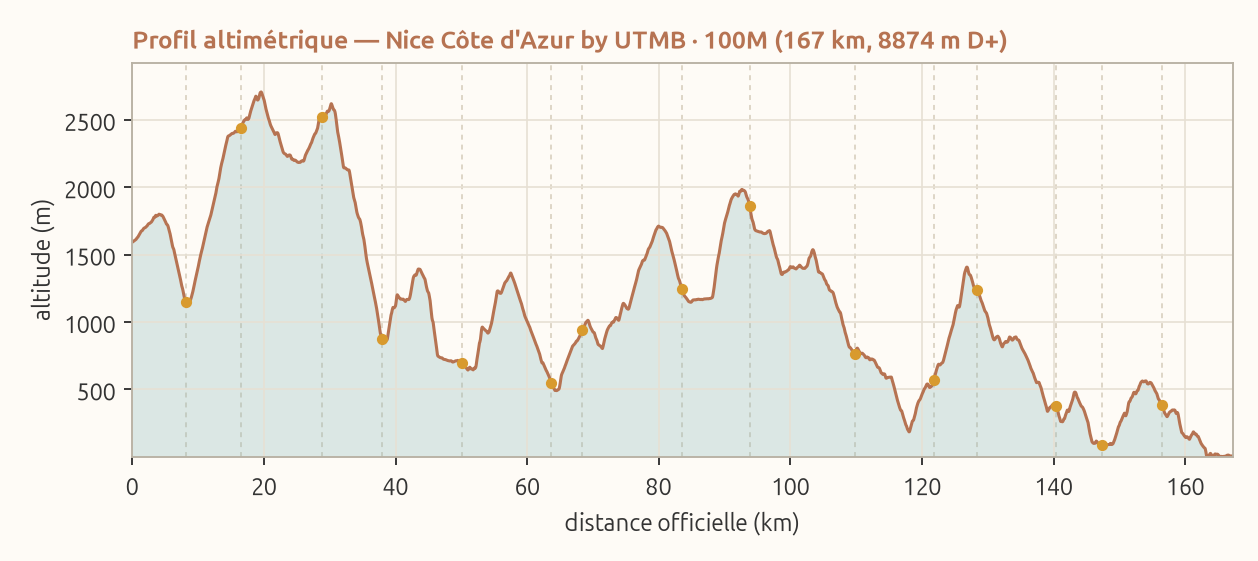
\includegraphics[width=\linewidth]{figures/profil.png}
  \caption{\`A lire : le relief r\'eel de ta course (8874\,m\,D+). Points dor\'es : les ravitaillements. Le plus dur monte vers \textbf{AS2 km16.5}.}
  \label{fig:profil}
\end{figure}

\subsection{Le co\^ut de la pente : la distance \'equivalente}
\emph{En clair :} courir un m\`etre en c\^ote co\^ute bien plus qu'un m\`etre \`a plat --- et une descente
raide co\^ute moins. On mesure ce co\^ut par la fonction de Minetti et~al.~\cite{minetti2002} :
\begin{equation}
C_r(i) = 155{,}4\,i^5 - 30{,}4\,i^4 - 43{,}3\,i^3 + 46{,}3\,i^2 + 19{,}5\,i + 3{,}6,
\label{eq:minetti}
\end{equation}
o\`u \(C_r\) vaut 3,6 \`a plat et \(f(i)=C_r(i)/3{,}6\) dit \og~combien de m\`etres \`a plat co\^ute un
m\`etre de pente \(i\)\,\fg.

\begin{llexemple}[Un exemple concret]
\`A \textbf{+15\,\% de pente}, courir un m\`etre \og~co\^ute~\fg\ comme \textbf{2,06\,m} \`a plat ; \`a \textbf{$-$15\,\%}, comme seulement \textbf{0,51\,m}. C'est pour \c{c}a qu'on ne raisonne pas en kilom\`etres bruts mais en \emph{distance \'equivalente \`a plat}.
\end{llexemple}

\begin{llnote}[Ce que \c{c}a change pour toi]
Tes 167\,km de montagne \og~p\`esent~\fg\ comme \textbf{200\,km \`a plat} : c'est ce chiffre, pas la distance affich\'ee, qui d\'etermine ton temps. Chaque mont\'ee que tu vois sur le profil est d\'ej\`a \og~convertie~\fg\ dans ce calcul.
\end{llnote}

En int\'egrant \(f\) le long du parcours, on obtient la \textbf{distance \'equivalente \`a plat}
\(\Deq \approx \textbf{200,1\,km}\). Le tableau~\ref{tab:demande} d\'etaille la demande de chaque
segment.

\begin{table}[H]
  \centering \scriptsize \setlength{\tabcolsep}{3.6pt}
  \LLzebra \renewcommand{\arraystretch}{1.3}
  \begin{tabular}{@{}clrrrrrrrr@{}}
    \LLheaderrow
    \LLthead{\#} & \LLthead{Ravitaillement} & \LLthead{dist.} & \LLthead{D+} & \LLthead{D--} & \LLthead{$\Deq$} & \LLthead{alt.} & \LLthead{$\Sigma$dist} & \LLthead{$\Sigma$D+} & \LLthead{$\Sigma$D--} \\
     & & \scriptsize(km) & \scriptsize(m) & \scriptsize(m) & \scriptsize(km) & \scriptsize(m) & \scriptsize(km) & \scriptsize(m) & \scriptsize(m) \\
    1 & AS1 km8.1 & \LLnum{8,1} & \LLnum{215} & \LLnum{656} & \LLnum{7,7} & \LLnum{1152} & \LLnum{8,1} & \LLnum{215} & \LLnum{656} \\
    2 & AS2 km16.5 & \LLnum{8,4} & \LLnum{1303} & \LLnum{19} & \LLnum{18,0} & \LLnum{2436} & \LLnum{16,5} & \LLnum{1518} & \LLnum{675} \\
    3 & AS3 km28.9 & \LLnum{12,4} & \LLnum{692} & \LLnum{608} & \LLnum{15,0} & \LLnum{2521} & \LLnum{28,9} & \LLnum{2210} & \LLnum{1282} \\
    4 & AS4 km38 & \LLnum{9,1} & \LLnum{108} & \LLnum{1757} & \LLnum{7,2} & \LLnum{872} & \LLnum{38,0} & \LLnum{2318} & \LLnum{3039} \\
    5 & AS5 km50.1 & \LLnum{12,1} & \LLnum{612} & \LLnum{788} & \LLnum{15,2} & \LLnum{695} & \LLnum{50,1} & \LLnum{2929} & \LLnum{3827} \\
    6 & AS6 km63.7 & \LLnum{13,6} & \LLnum{807} & \LLnum{953} & \LLnum{16,3} & \LLnum{549} & \LLnum{63,7} & \LLnum{3736} & \LLnum{4781} \\
    7 & AS7 km68.4 & \LLnum{4,7} & \LLnum{453} & \LLnum{59} & \LLnum{7,6} & \LLnum{942} & \LLnum{68,4} & \LLnum{4189} & \LLnum{4840} \\
    8 & AS8 km83.5 & \LLnum{15,1} & \LLnum{1048} & \LLnum{748} & \LLnum{19,9} & \LLnum{1242} & \LLnum{83,5} & \LLnum{5237} & \LLnum{5588} \\
    9 & AS9 km93.8 & \LLnum{10,3} & \LLnum{868} & \LLnum{250} & \LLnum{16,1} & \LLnum{1861} & \LLnum{93,8} & \LLnum{6106} & \LLnum{5838} \\
    10 & AS10 km109.8 & \LLnum{16,0} & \LLnum{267} & \LLnum{1367} & \LLnum{13,6} & \LLnum{761} & \LLnum{109,8} & \LLnum{6373} & \LLnum{7205} \\
    11 & AS11 km121.8 & \LLnum{12,0} & \LLnum{491} & \LLnum{682} & \LLnum{12,8} & \LLnum{570} & \LLnum{121,8} & \LLnum{6864} & \LLnum{7887} \\
    12 & AS12 km128.3 & \LLnum{6,5} & \LLnum{855} & \LLnum{188} & \LLnum{12,3} & \LLnum{1237} & \LLnum{128,3} & \LLnum{7718} & \LLnum{8075} \\
    13 & AS13 km140.4 & \LLnum{12,1} & \LLnum{196} & \LLnum{1056} & \LLnum{9,7} & \LLnum{376} & \LLnum{140,4} & \LLnum{7914} & \LLnum{9131} \\
    14 & AS14 km147.4 & \LLnum{7,0} & \LLnum{249} & \LLnum{539} & \LLnum{7,0} & \LLnum{87} & \LLnum{147,4} & \LLnum{8163} & \LLnum{9670} \\
    15 & AS15 km156.5 & \LLnum{9,1} & \LLnum{537} & \LLnum{242} & \LLnum{11,8} & \LLnum{382} & \LLnum{156,5} & \LLnum{8701} & \LLnum{9912} \\
    16 & Arrivée Nice km167.2 & \LLnum{10,7} & \LLnum{173} & \LLnum{549} & \LLnum{9,9} & \LLnum{6} & \LLnum{167,2} & \LLnum{8874} & \LLnum{10461} \\
  \end{tabular}
  \caption{Demande de chaque segment. Colonnes $\Sigma$ : cumuls depuis le d\'epart. \(\Deq\) : distance \'equivalente \`a plat.}
  \label{tab:demande}
\end{table}

Deux segments ressortent : la \textbf{plus grosse mont\'ee} vers \textbf{AS2 km16.5} (+1303\,m, pente moyenne 16\,\%), et la \textbf{plus grosse descente} vers \textbf{AS4 km38} ($-$1757\,m). Ce sont eux qui structurent l'effort.

\begin{figure}[H]
  \centering
  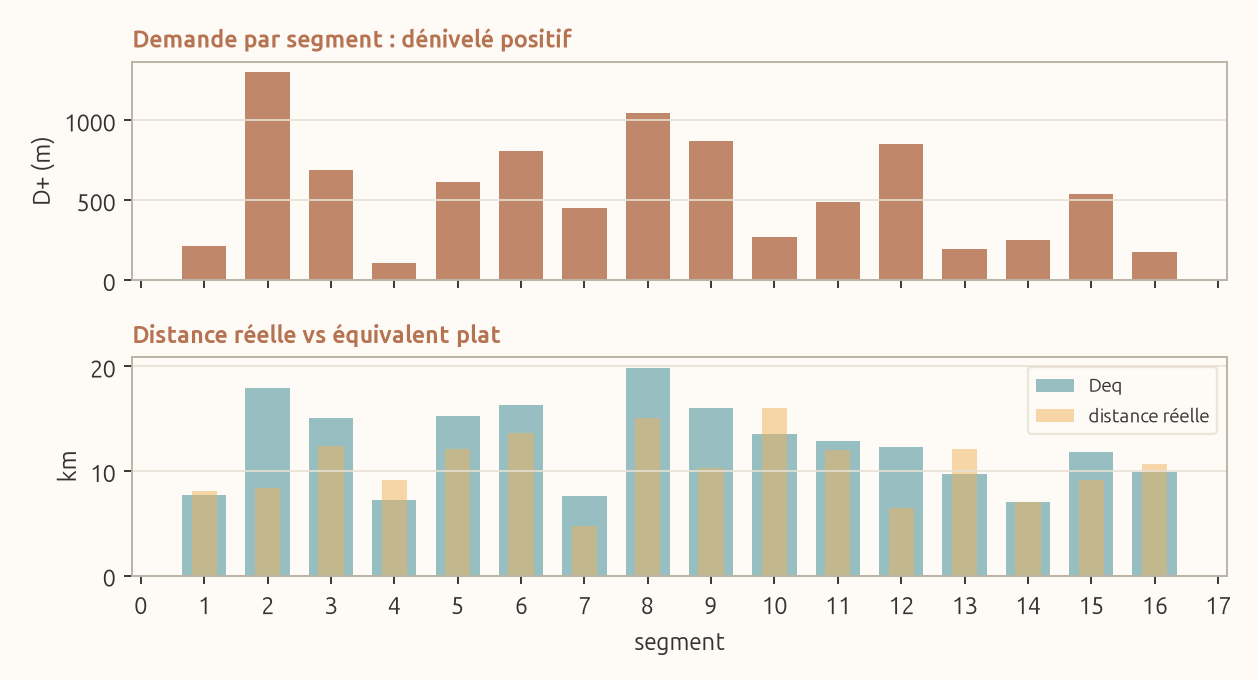
\includegraphics[width=\linewidth]{figures/demande.png}
  \caption{\`A lire : en haut, le d\'enivel\'e positif par segment ; en bas, distance r\'eelle vs \'equivalent plat. L'\'ecart entre les deux barres, c'est la \og~taxe~\fg\ de la pente.}
  \label{fig:demande}
\end{figure}

% =====================================================================
\section{Ton jumeau num\'erique}
Le \emph{jumeau}, c'est le r\'esum\'e chiffr\'e de tes capacit\'es, extrait de 419~activit\'es.

\subsection{Volume d'entra\^inement r\'ecent}
Tes 4~derni\`eres semaines de donn\'ees (\textbf{350\,km} et
\textbf{18\,201\,m\,D+} au total). La pr\'ediction suppose ta \emph{forme du moment} :
si l'export date d'avant la course, ces volumes sont \`a recalculer \`a l'approche.
\begin{table}[H]
  \centering \footnotesize
  \LLzebra \renewcommand{\arraystretch}{1.25}
  \begin{tabular}{@{}lrrr@{}}
    \LLheaderrow
    \LLthead{Semaine} & \LLthead{distance} & \LLthead{D+} & \LLthead{sorties} \\
     & \footnotesize(km) & \footnotesize(m) & \\
    26/05–01/06 & \LLnum{94} & \LLnum{4488} & \LLnum{7} \\
    02/06–08/06 & \LLnum{102} & \LLnum{7143} & \LLnum{5} \\
    09/06–15/06 & \LLnum{59} & \LLnum{2835} & \LLnum{7} \\
    16/06–22/06 & \LLnum{96} & \LLnum{3735} & \LLnum{6} \\
  \end{tabular}
  \caption{Volume hebdomadaire r\'ecent (distance brute et d\'enivel\'e positif).}
  \label{tab:volume}
\end{table}

\subsection{Vitesse critique et courbe record}
\emph{En clair :} ta \textbf{vitesse critique} (VC) est la fronti\`ere entre \og~je peux tenir
longtemps~\fg\ et \og~\c{c}a br\^ule~\fg. On l'estime en ajustant \(d = \VC\cdot t + D'\) sur tes
efforts plats \og~propres~\fg~\cite{poole2016,jones2017} :
\begin{equation}
\boxed{\;\VC = (2,845 \pm 0,20)~\mathrm{m\,s^{-1}} \;=\; 10,24~\mathrm{km\,h^{-1}} \;=\; 5:51~\mathrm{min/km}\;}
\end{equation}

\begin{figure}[H]
  \centering
  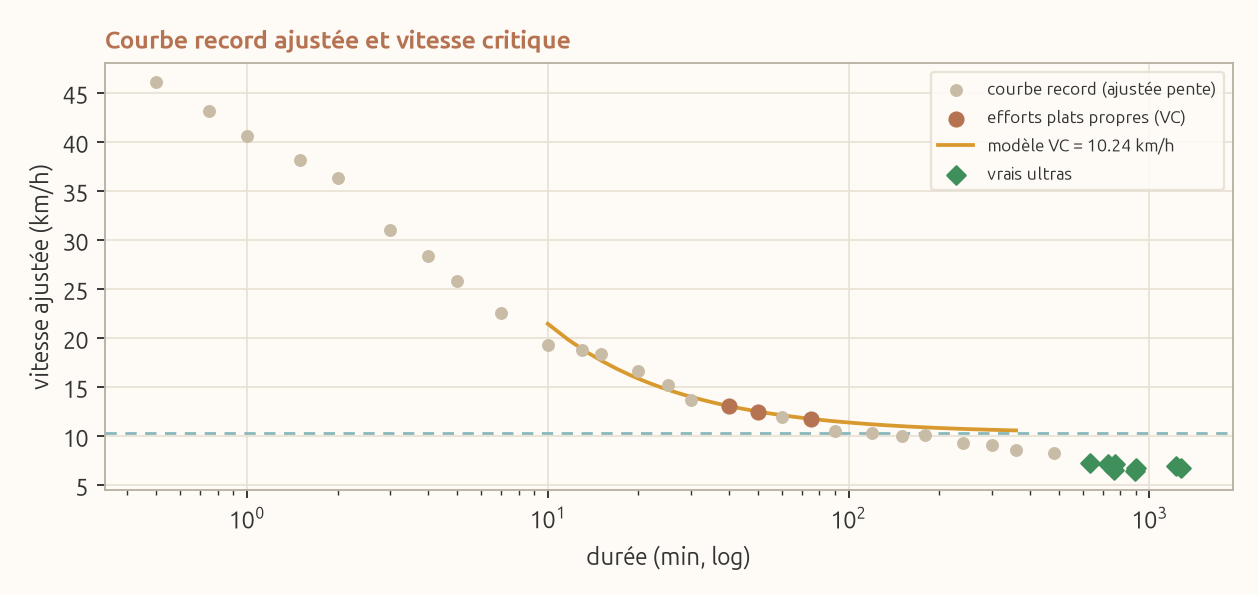
\includegraphics[width=\linewidth]{figures/record.png}
  \caption{\`A lire : pour chaque dur\'ee, ta meilleure vitesse ajust\'ee \`a la pente. Les efforts plats \og~propres~\fg\ (terracotta) calent la vitesse critique ; les losanges verts sont tes vrais ultras. Ils tournent \`a \textbf{67\,\%} de ta VC : un ultra se court tr\`es loin sous le plafond.}
  \label{fig:record}
\end{figure}

\begin{llnote}[Ce que \c{c}a change pour toi]
Ta vitesse critique (\textasciitilde{}10,2\,km/h) est ton \textbf{seuil} : au-dessus, l'effort se paie vite ; en dessous, tu peux tenir longtemps. Sur cet ultra tu cours \`a \textbf{64\,\%} de cette VC — tr\`es loin du plafond : garde de la marge, surtout au d\'epart.
\end{llnote}

\begin{llattention}[Une honn\^etet\'e m\'ethodologique]
Les efforts \emph{courts} (< 30\,min), presque toujours en c\^ote, sont \'ecart\'es de l'estimation de
la VC : l'ajustement de pente surestime alors la vitesse \'equivalente. Sans cons\'equence pour un ultra,
couru tr\`es loin sous la VC.
\end{llattention}

\subsection{Exposant d'endurance et durabilit\'e}
En clair : c'est ta capacit\'e \`a \textbf{garder de la vitesse quand la dur\'ee s'allonge}. Plus l'exposant est \'elev\'e, plus ton moteur est taill\'e pour le tr\`es long. On l'obtient par une loi de puissance \(v \propto t^{-\alpha}\) sur l'enveloppe
longue, d'o\`u l'exposant de Riegel \(E = 1/(1-\alpha)\)~\cite{riegel1981,drake2024}.
\begin{llnote}[Ce que \c{c}a change pour toi]
Ton exposant vaut \textbf{1,22} — c'est un atout majeur sur un ultra : tu d\'eclines peu par rapport \`a ta vitesse de base.
\end{llnote}

\emph{En clair :} la \textbf{durabilit\'e}, c'est ta r\'esistance \`a l'usure --- mesur\'ee par le
\og~d\'ecouplage~\fg, l'\'ecart d'efficacit\'e (allure pour une FC donn\'ee) entre la premi\`ere et la
seconde moiti\'e de tes longues sorties~\cite{maunder2021,jones2024}.
\begin{llnote}[Ce que \c{c}a change pour toi]
\textbf{21\,\%} de d\'ecouplage : la d\'erive contr\^ol\'ee du plan est faite pour toi : pars sans t'emballer. C'est l'un des deux vrais facteurs limitants d'un ultra (avec le ravitaillement).
\end{llnote}

% =====================================================================
\section{Pr\'ediction et validation}\label{sec:pred}
\emph{En clair :} plus tu cours longtemps, plus tu ralentis --- mais ta dur\'ee d\'epend justement de ta
vitesse. On r\'esout ce cercle par un \textbf{point fixe} \(T = \Deq / v(T)\). Pour l'incertitude, on fait
un \textbf{Monte-Carlo} : on \emph{simule des milliers de courses possibles} en tirant ta vitesse au hasard
dans sa plage probable (de dispersion \(\sigma = 0,22\)~\(\mathrm{km\,h^{-1}}\)). R\'esultat :
\textbf{30\,h\,44}, intervalle 80\,\% \textbf{29\,h\,29 -- 32\,h\,09}.

\begin{llnote}[Lire l'intervalle \`a 80\,\%]
Compte tenu de l'incertitude du mod\`ele, il y a \textbf{80\,\% de chances} que ton temps r\'eel tombe
dans cette fourchette --- environ 1~chance sur 10 d'\^etre plus rapide que la borne basse, 1~sur~10 d'\^etre
plus lent. La valeur centrale reste le sc\'enario le plus probable.
\end{llnote}

\begin{llnote}[Ce que \c{c}a change pour toi]
Vise \textbf{30\,h\,44}. \`A cette intensit\'e, ce n'est pas une question de vitesse pure mais d'\textbf{ex\'ecution} : r\'egularit\'e, ravitaillement, gestion des descentes. La fourchette dit l'incertitude, pas un objectif \`a battre. Au d\'epart, \c{c}a doit te para\^itre \textbf{trop facile}. C'est normal et voulu : \`a cette intensit\'e, l'erreur classique est de partir trop vite. Retiens-toi.\end{llnote}

\emph{En clair :} pour savoir si on peut te faire confiance, on a rejou\'e la pr\'ediction
sur chacun de tes ultras pass\'es \emph{en l'excluant} du calcul (validation crois\'ee leave-one-out).

\begin{figure}[H]
  \centering
  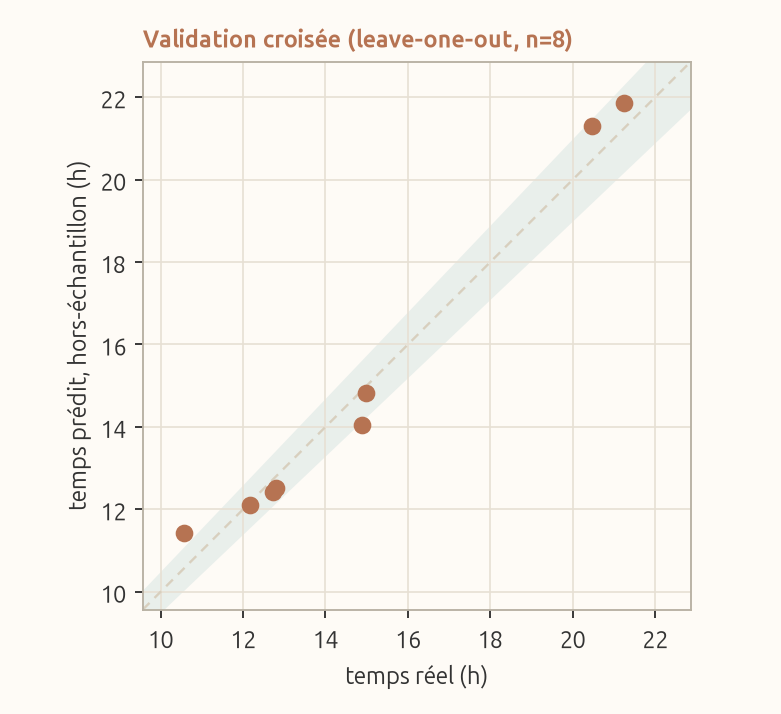
\includegraphics[width=0.62\linewidth]{figures/validation.png}
  \caption{\`A lire : chaque point est un de tes ultras, pr\'edit \emph{sans lui}. Plus c'est proche de la diagonale, mieux la m\'ethode te conna\^it. Ici, \`a \textbf{3,4\,\%} pr\`es en moyenne (bande $\pm$5\,\%).}
  \label{fig:validation}
\end{figure}

\begin{llnote}[Ce que \c{c}a change pour toi]
On a re-pr\'edit chacun de tes ultras pass\'es \emph{sans lui}, puis compar\'e au r\'eel : en moyenne \textbf{3,4\,\%} d'\'ecart. Autrement dit, la m\'ethode s'est d\'ej\`a \textbf{prouv\'ee sur toi} — ce n'est pas une promesse en l'air.
\end{llnote}

% =====================================================================
\section{Le plan de pacing}

\textbf{Effort ajust\'e constant.} On vise une \textbf{vitesse ajust\'ee \`a la pente} (\'equivalent
plat) constante, et non une allure r\'eelle constante : courir au m\^eme \emph{co\^ut m\'etabolique}
impose de ralentir en mont\'ee et d'acc\'el\'erer en descente. \textbf{Fade de durabilit\'e.} Comme la
durabilit\'e d\'ecline avec les heures, on autorise une l\'eg\`ere \textbf{d\'erive} --- une baisse
progressive de cette vitesse du d\'ebut \`a la fin (\(\approx -16\,\%\)) : partir un peu
au-dessus de la moyenne, finir un peu en dessous. Les \textbf{fen\^etres} donnent par segment une \emph{plage} d'arriv\'ee
(bandes Monte-Carlo), pas une valeur unique.

\begin{table}[H]
  \centering \scriptsize \setlength{\tabcolsep}{3.8pt}
  \LLzebra \renewcommand{\arraystretch}{1.28}
  \begin{tabular}{@{}clrrrrlrc@{}}
    \LLheaderrow
    \LLthead{\#} & \LLthead{Vers} & \LLthead{km} & \LLthead{$\Deq$} & \LLthead{v.aj.} & \LLthead{allure} & \LLthead{arriv\'ee} & \LLthead{fen.(h)} & \LLthead{nuit} \\
     & & & \scriptsize(km) & \scriptsize(km/h) & \scriptsize(/km) & & & \\
    1 & AS1 km8.1 & \LLnum{8,1} & \LLnum{7,7} & \LLnum{7,48} & \LLnum{7:37} & ven. 14:06 & \LLnum{1,1–1,2} &  \\
    2 & AS2 km16.5 & \LLnum{16,5} & \LLnum{18,0} & \LLnum{7,41} & \LLnum{17:19} & ven. 16:37 & \LLnum{3,5–3,8} &  \\
    3 & AS3 km28.9 & \LLnum{28,9} & \LLnum{15,0} & \LLnum{7,31} & \LLnum{9:57} & ven. 18:45 & \LLnum{5,5–6,0} &  \\
    4 & AS4 km38 & \LLnum{38,0} & \LLnum{7,2} & \LLnum{7,25} & \LLnum{6:34} & ven. 19:50 & \LLnum{6,6–7,2} & $\bullet$ \\
    5 & AS5 km50.1 & \LLnum{50,1} & \LLnum{15,2} & \LLnum{7,18} & \LLnum{10:31} & ven. 22:12 & \LLnum{8,8–9,6} & $\bullet$ \\
    6 & AS6 km63.7 & \LLnum{63,7} & \LLnum{16,3} & \LLnum{7,09} & \LLnum{10:08} & sam. 00:35 & \LLnum{11,1–12,1} & $\bullet$ \\
    7 & AS7 km68.4 & \LLnum{68,4} & \LLnum{7,6} & \LLnum{7,02} & \LLnum{13:49} & sam. 01:45 & \LLnum{12,2–13,3} & $\bullet$ \\
    8 & AS8 km83.5 & \LLnum{83,5} & \LLnum{19,9} & \LLnum{6,94} & \LLnum{11:24} & sam. 04:42 & \LLnum{15,1–16,4} & $\bullet$ \\
    9 & AS9 km93.8 & \LLnum{93,8} & \LLnum{16,1} & \LLnum{6,83} & \LLnum{13:41} & sam. 07:18 & \LLnum{17,6–19,1} & $\bullet$ \\
    10 & AS10 km109.8 & \LLnum{109,8} & \LLnum{13,6} & \LLnum{6,74} & \LLnum{7:33} & sam. 09:24 & \LLnum{19,6–21,3} &  \\
    11 & AS11 km121.8 & \LLnum{121,8} & \LLnum{12,8} & \LLnum{6,67} & \LLnum{9:38} & sam. 11:24 & \LLnum{21,5–23,4} &  \\
    12 & AS12 km128.3 & \LLnum{128,3} & \LLnum{12,3} & \LLnum{6,59} & \LLnum{17:16} & sam. 13:31 & \LLnum{23,5–25,6} &  \\
    13 & AS13 km140.4 & \LLnum{140,4} & \LLnum{9,7} & \LLnum{6,53} & \LLnum{7:22} & sam. 15:05 & \LLnum{25,0–27,3} &  \\
    14 & AS14 km147.4 & \LLnum{147,4} & \LLnum{7,0} & \LLnum{6,48} & \LLnum{9:19} & sam. 16:16 & \LLnum{26,2–28,5} &  \\
    15 & AS15 km156.5 & \LLnum{156,5} & \LLnum{11,8} & \LLnum{6,42} & \LLnum{12:06} & sam. 18:11 & \LLnum{28,0–30,5} &  \\
    16 & Arrivée Nice km167.2 & \LLnum{167,2} & \LLnum{9,9} & \LLnum{6,36} & \LLnum{8:43} & sam. 19:44 & \LLnum{29,5–32,1} & $\bullet$ \\
  \end{tabular}
  \caption{Plan par segment : vitesse ajust\'ee cible, allure r\'eelle terrain, heure de passage et
  fen\^etre d'arriv\'ee (80\,\%). $\bullet$ = section de nuit.}
  \label{tab:plan}
\end{table}

Total : mouvement 28\,h\,59 + arr\^ets 1\,h\,45 = horloge \textbf{30\,h\,44}.
 Soleil : lever 07:20, coucher 19:24.
\begin{figure}[H]
  \centering
  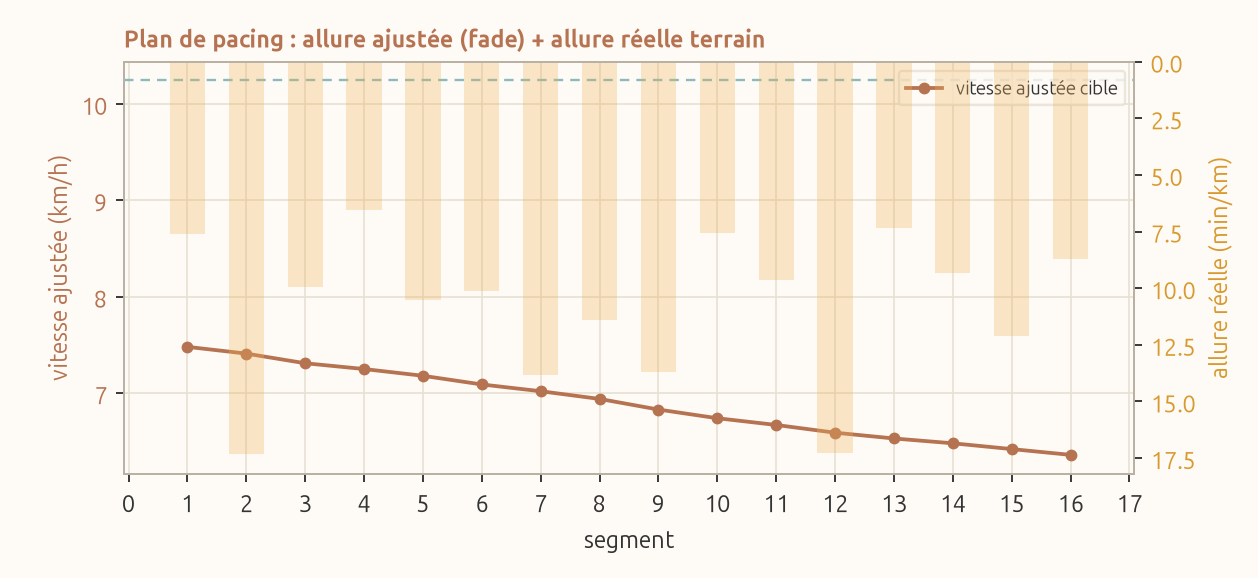
\includegraphics[width=\linewidth]{figures/pacing.png}
  \caption{\`A lire : en terracotta, ta \textbf{vitesse ajust\'ee cible} (effort constant, l\'eg\`ere d\'erive) ; en barres, l'\textbf{allure r\'eelle} sur le terrain — lente en mont\'ee, rapide en descente, pour un \emph{m\^eme} co\^ut.}
  \label{fig:pacing}
\end{figure}

\begin{figure}[H]
  \centering
  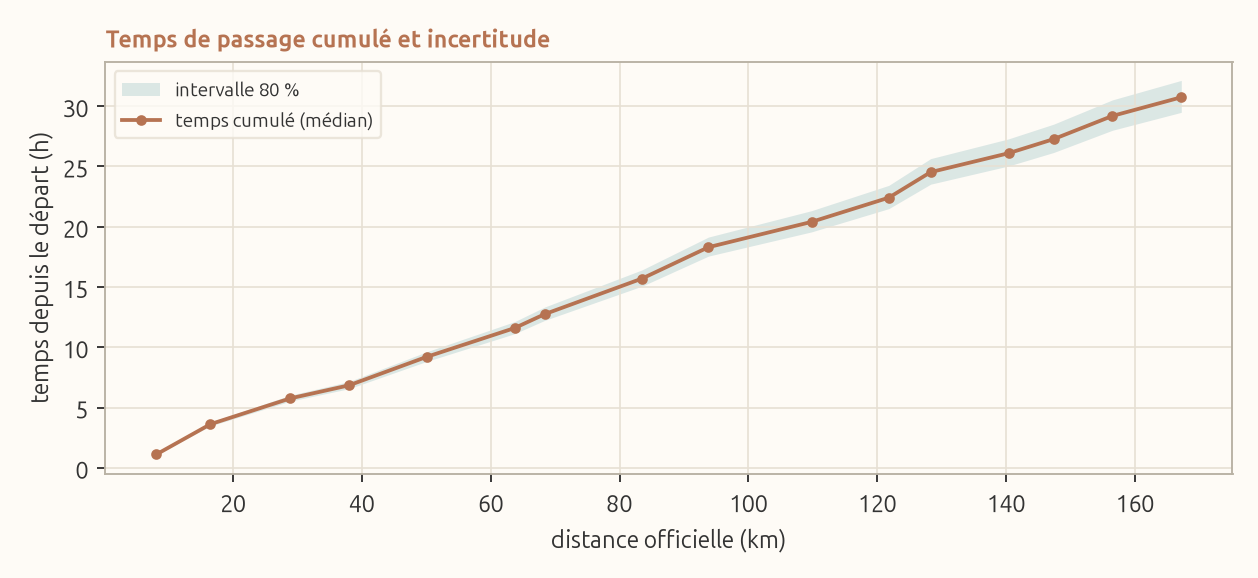
\includegraphics[width=\linewidth]{figures/cumul.png}
  \caption{\`A lire : ton heure de passage cumul\'ee. La bande, c'est la \textbf{fourchette \`a 80\,\%} : large vers la fin, car les incertitudes s'additionnent au fil des heures.}
  \label{fig:cumul}
\end{figure}

% =====================================================================
\section{Strat\'egie de course}
Concr\`etement, voici o\`u se gagne (ou se perd) ta course --- d\'eduit de \emph{ton} parcours et de
\emph{ton} plan :
\begin{itemize}[leftmargin=1.4em]
\item \textbf{\'Eclairage et nuit.} Section de nuit autour du \textbf{km\,38 au km\,94} (ven. 19:50 \`a sam. 07:18) : frontale charg\'ee \textbf{+ batterie/pile de rechange}, et de quoi avoir chaud (la temp\'erature chute la nuit, surtout en altitude).
\item \textbf{Discipline dans la plus grosse mont\'ee.} Vers \textbf{AS2 km16.5} (+1303\,m \`a 16\,\%) : \textbf{garde de la marge}, marche d\`es que \c{c}a devient raide (souvent plus efficace que courir), et ne \og~grille pas d'allumettes~\fg\ ici — la course se gagne plus loin.
\item \textbf{Protection des quadriceps en descente.} La plus grosse descente m\`ene vers \textbf{AS4 km38} ($-$1757\,m) : \textbf{foul\'ee courte}, cadence \'elev\'ee, contr\^ole. C'est l\`a que se joue la casse musculaire qui peut ruiner la fin de course — m\^eme si tu te sens bien, retiens-toi.
\item \textbf{Ravitaillement.} Le ravitaillement est l'\textbf{autre} facteur limitant : mange et bois \textbf{avant} d'avoir faim ou soif, r\'eguli\`erement. Un creux \'energ\'etique co\^ute bien plus cher que les minutes pass\'ees \`a un ravito.
\end{itemize}

% =====================================================================
\section{Limites assum\'ees}
Un plan n'est utile que si l'on sait \emph{ce qu'il ne capture pas}.
\begin{llattention}[\`A garder en t\^ete]
\begin{itemize}[leftmargin=1.4em]
\item \textbf{Forme du jour} : si tes donn\'ees s'arr\^etent avant la course, la pr\'ediction suppose la
forme du moment et doit \^etre recalcul\'ee \`a l'approche.
\item \textbf{Allures de descente} = plafonds m\'etaboliques ; la \textbf{technicit\'e} du terrain (absente
du GPX) peut imposer plus lent.
\item \textbf{Minetti} perd en validit\'e au-del\`a de \(\pm\)25--30\,\% \textbf{de pente} (marche active).
\item \textbf{M\'et\'eo} et \textbf{nutrition} ne sont pas mod\'elis\'ees.
\end{itemize}
\end{llattention}

\begin{llnote}[Glossaire express]
\textbf{Vitesse critique (VC)} --- ton seuil d'effort soutenable : au-dessus, la fatigue s'accumule vite.\par
\textbf{R\'eserve $D'$} --- ta petite \og~r\'eserve~\fg\ au-del\`a de la VC, pour les efforts courts (sans impact en ultra).\par
\textbf{Distance \'equivalente \`a plat ($\Deq$)} --- tes kilom\`etres de montagne convertis en kilom\`etres \`a plat \'equivalents en effort.\par
\textbf{Exposant d'endurance} --- \`a quelle vitesse ton allure soutenable baisse quand la dur\'ee s'allonge.\par
\textbf{Durabilit\'e / d\'ecouplage} --- la perte d'efficacit\'e (allure pour une FC donn\'ee) en fin de longue sortie.\par
\textbf{Pr\'ediction auto-coh\'erente (point fixe)} --- ta vitesse d\'epend de la dur\'ee, qui d\'epend de ta vitesse : on r\'esout les deux ensemble.\par
\textbf{Validation crois\'ee (leave-one-out)} --- rejouer la pr\'ediction sur chaque ultra pass\'e \emph{en l'excluant}, pour mesurer l'erreur r\'eelle.\par
\end{llnote}

% =====================================================================
\printbibliography[heading=bibintoc, title={R\'ef\'erences}]

\end{document}